In this section we will discuss a number of methods used for model checking timed automata. We will choose a method which we will use for the rest of this project.

\subsection{Methods}
Already several model checkers for timed automata exist, such as \uppaal{}~\cite{UPPAAL}, KRONOS~\cite{kronos}, RABBIT~\cite{CAV03} and RED~\cite{crds}. We focus mainly on the \uppaal{} tool as we use the same input format. Opaal~\cite{opaal}, the language module for \ltsmin{}, uses the XML format that is created by the \uppaal{} tools. This way we can use the \uppaal{} user interface to create and adapt models. We also use the \uppaal{} DBM library to represent zones.

The most established method to represent clock zones are DBMs. We gave an introduction to this structure in the preliminaries section. Several diagrams based on BDDs have been developed to represent zones. All of these are similar to DBMs in the sense that they use clock constraints to represent the zones. The structure of these diagrams is BDD-like to represent the zones more efficiently. Below we shortly describe four zone based methods. For each method we give an example, all examples represent $2 < c_1 - c_2 < 4 \vee 7 \leq c_1 - c_2 \leq 8$. This is a non-convex zone, and consequently cannot be represented by a single DBM. The representing zone is drawn in Figure \ref{fig:symbolic-example}

\begin{figure}[h]
\centering
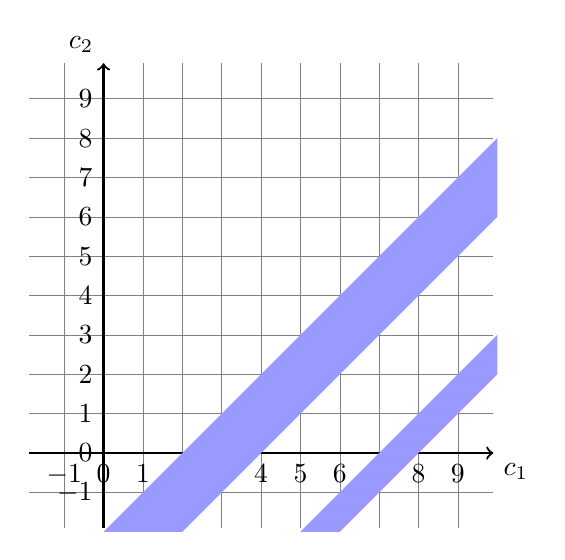
\begin{tikzpicture}[scale=0.5]

\draw[step=1cm,gray,very thin] (-1.9,-1.9) grid (9.9,9.9);
\draw[thick,->] (-1.9,0) -- (9.9,0) node[anchor=north west] {$c_1$};
\draw[thick,->] (0,-1.9) -- (0,9.9) node[anchor=south east] {$c_2$};

\foreach \x in {-1,0,1,2,3,4,5,6,7,8,9}
    \draw (\x cm,1pt) -- (\x cm,-1pt) node[anchor=north] {$\x$};
\foreach \y in {-1,0,1,2,3,4,5,6,7,8,9}
    \draw (1pt,\y cm) -- (-1pt,\y cm) node[anchor=east] {$\y$};

\fill[fill=blue!40!white] (5,-2) -- (10,3) -- (10,2) -- (6,-2) -- (5,-2);

\fill[fill=blue!40!white] (0,-2) -- (2,-2) -- (10,6) -- (10,8) -- (0,-2);
    
%\filldraw[fill=blue!40!white, draw=black] (0,0) rectangle (5,5);
\end{tikzpicture}
\caption{Zone represented by the examples for all symbolic approaches}
\label{fig:symbolic-example}
\end{figure}

\subsubsection{Clock Difference Diagram}
CDDs~\cite{BRICS19491} use single nodes for each variable and have multiple edges each containing a disjoint interval of that variable. This results into a node with a larger fanout. The upper and lower bound for each pair of clocks are represented in a single node, as the edges represent intervals. Requiring the disjointness of intervals can lead to a memory inefficient representation, as intervals need to be cut into smaller parts. All algorithms on CDDs do not maintain disjointness, after every step it needs to be re-established. In Figure \ref{fig:cdd-example} we have an example of a CDD.

\begin{mydef}[Clock Difference Diagram~\cite{BRICS19491}]
A clock difference diagram is defined as a directed, acyclic graph, which has
\begin{itemize}
\item a node called the start node from which all nodes of the graph are reachable
\item inner nodes written as $((i,j),(I_1,,T_1,...,(I_q,T_q))$ where $(i,j)$ is the pair of clocks of the constraint, the $I_n$ are intervals of the real numbers, and the $T_n$ are CDDs again. We require completeness, i.e. $\bigcup_{n\in \{1,...,q\}}I_n= \mathbb{R}$
\item end-nodes which are either TRUE or FALSE
\end{itemize}

\end{mydef}

\begin{figure}[h]
\begin{center}
	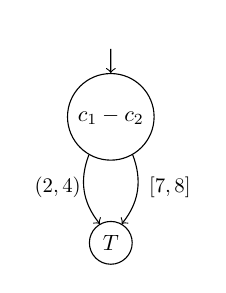
\begin{tikzpicture}[
		smallvertex/.style={circle,draw,scale=0.8}
		]
			
		\node[smallvertex](S0){$c_1 - c_2$};
	    \node[smallvertex, draw = none, above of = S0, yshift = 0.25cm](S4){};
		\draw[->] (S4) --(S0) node [midway, above, sloped, scale=0.75,
		rotate=295, xshift =-0.4 cm, yshift = -0.2cm]{};
		\node[smallvertex, below of = S0, yshift = -1cm](S3){$T$};
		\draw[->] (S0) edge [bend left](S3) node [midway, above, sloped, scale=0.75,
		rotate=0, xshift =-0.9 cm, yshift = -1.5cm]{$(2,4)$};
		\draw[->] (S0) edge [bend right](S3) node [midway, above, sloped, scale=0.75,
		rotate=0, xshift =1 cm, yshift = -1.5cm]{$[7,8]$};
	\end{tikzpicture}
\end{center}
\caption{CDD representation}
\label{fig:cdd-example}
\end{figure}

\subsubsection{Difference Decision Diagram}
DDDs~\cite{ddds, ddd-datastructure-99} use an upper-bound clock constraint for a variable pair on each node that can either be true or false. Each node, thus has a fixed fanout of two, a true and a false edge. When a constraint is false, a next node will have another constraint on the same variable, a true edge will go down to the next level with constraints over another pair of variables. This requires a fixed ordering based on the variables, values and operators. The apply operator that is defined over DDDs has the same complexity as that over BDDs. In Figure \ref{fig:ddd-example} an example of a DDD is shown.

\begin{mydef}[Difference Decision Diagram~\cite{ddds}]
\label{def:DDD}
A difference decision diagram (DDD) is a directed acyclic graph $(V,E)$. The vertex set $V$ contains two terminals $0$ and $1$ with out-degree zero, and a set of non-terminal vertices with out-degree two and the following attributes.
\\\\
\begin{tabular}{lll}
Attribute                & Type                      & Description                                           \\\hline
pos(v), neg(v)           & \textbf{Var}              & Positive variable $x_i$, and negative variable $x_j$. \\
op(v)                    & $\{<$, $\leq\}$     & Operator $<$ or $\leq$.                         \\
const(v)                 & $\mathbb{D}$              & Constant c.                                           \\
high(v), low(v)          & $V$                       & High-branch h, and low-branch l.                   
\end{tabular}
\captionof*{table}{}  
The set E contains the edges $(v,low(v))$ and $(v, high(v))$, where $v \in V$ is a non-terminal vertex.
\end{mydef}

\begin{figure}[h]
\begin{center}
	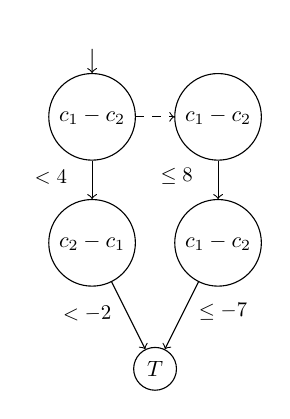
\begin{tikzpicture}[
		smallvertex/.style={circle,draw,scale=0.8}
		]
			
		\node[smallvertex](S0){$c_1 - c_2$};
		\node[smallvertex, draw = none, above of = S0, yshift = 0.25cm](S5){};
		\draw[->] (S5) --(S0) node [midway, above, sloped, scale=0.75,
		rotate=295, xshift =-0.4 cm, yshift = -0.2cm]{};
		\node[smallvertex, right of = S0, xshift = 1cm](S1){$c_1 - c_2$};
		\draw[dashed,->] (S0) --(S1) node [midway, above, sloped, scale=0.75,
		rotate=0, xshift =-0.7 cm, yshift = -0.2cm]{};
		\node[smallvertex, below of = S0, yshift = -1cm](S2){$c_2 - c_1$};
		\draw[->] (S0) --(S2) node [midway, above, sloped, scale=0.75,
		rotate=90, xshift =-0.7 cm, yshift = -0.2cm]{$< 4$};
		\node[smallvertex, below of = S1, yshift = -1cm](S3){$c_1 - c_2$};
		\draw[->] (S1) --(S3) node [midway, above, sloped, scale=0.75,
		rotate=90, xshift =-0.7 cm, yshift = -0.2cm]{$\leq 8$};
		\node[smallvertex, below of = S0, xshift = 1cm, yshift = -3cm](S4){$T$};
		\draw[->] (S2) --(S4) node [midway, above, sloped, scale=0.75,
		rotate=65, xshift =-0.7 cm, yshift = -0.2cm]{$<-2$};
		\draw[->] (S3) --(S4) node [midway, above, sloped, scale=0.75,
		rotate=297, xshift =0.7 cm, yshift = -0.2cm]{$\leq-7$};
	\end{tikzpicture}
\end{center}
\caption{DDD representation}
\label{fig:ddd-example}
\end{figure}

\subsubsection{Clock Restriction Diagram}
CRDs~\cite{crds} differ mainly from CDDs by not using disjoint intervals but possibly overlapping upper bounds, for a pair of variables on their edges. This diagram will have a larger fanout per node, like CDDs. Several normal forms for this diagram are proposed, with different performance results. The results of CRDs have been compared to CDDs. Results were sometimes exponentially better, in other cases linear worse than CDDs, this due to the fact that each variable pair needs a node for both their upper and lower bound, where CDDs fit this in a single node. It is also shown that CRDs can be combined with BDDs into a single structure to fully symbolically represent the state space. In Figure \ref{fig:crd-example} we give an example of a CRD.
\begin{mydef}[Clock Restriction Diagram~\cite{crds}]
Given a set of variables $V=\{x-x'|x,x'\in X \cup \{0\}\}\cup \{true\}$, an evaluation index $\Omega$ over $V$, and a timing constant $C_A$, a CRD over $V, \Omega$, and $C_A$ is a tuple $D = (v,(\beta_1,D_1),...,(\beta_n,D_n))$ with $n  \geq 0$ and $v \in V$ such that
\begin{itemize}
\item $v = true$ iff $n=0$
\item if $v \neq true$, then for all $1 \leq i \leq n, \beta_i \in B_{C_A}$ and $D_i$ is a CRD, say $(v_i,(\beta_{i,1},D_{i,1}),...,(\beta_{i,m},D_{i,m}))$, over $V, \Omega$, and $C_A$ with $v \prec_\Omega v_i$
\item if $v \neq true$, then for all $1 \leq i < j \leq n$, $\beta_i \neq \beta_j$
\item if $v \neq true$ and $n = 1$, then $\beta_1 \neq (<,\infty)$
\end{itemize}
\end{mydef}

\begin{figure}[h]
\begin{center}
	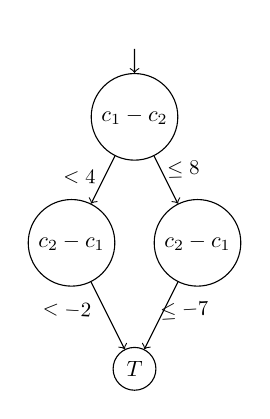
\begin{tikzpicture}[
		smallvertex/.style={circle,draw,scale=0.8}
		]
		\node[smallvertex](S0){$c_1 - c_2$};
		\node[smallvertex, draw = none, above of = S0, yshift = 0.25cm](S4){};
		\draw[->] (S4) --(S0) node [midway, above, sloped, scale=0.75,
		rotate=295, xshift =-0.4 cm, yshift = -0.2cm]{};
		\node[smallvertex, below of = S0, yshift = -1 cm, xshift = -1 cm](S1){$c_2 - c_1$};
		\node[smallvertex, below of = S0, yshift = -1 cm, xshift = 1  cm](S2){$c_2 - c_1$};
		\draw[->] (S0) --(S1) node [midway, above, sloped, scale=0.75,
		rotate=295, xshift =-0.4 cm, yshift = -0.2cm]{$<4$};
		\draw[->] (S0) --(S2) node [midway, above, sloped, scale=0.75,
		rotate=65, xshift =0.3 cm, yshift = -0.1cm]{$\leq 8$};
		\node[smallvertex, below of = S0, yshift = -3cm](S3){$T$};
		\draw[->] (S1) --(S3) node [midway, above, sloped, scale=0.75,
		rotate=60, xshift =-0.7 cm, yshift = -0.2cm]{$<-2$};
		\draw[->] (S2) --(S3) node [midway, above, sloped, scale=0.75,
		rotate=300, xshift =0.4 cm, yshift = -0.2cm]{$\leq-7$};
	\end{tikzpicture}
\end{center}
\caption{CRD representation}
\label{fig:crd-example}
\end{figure}

\subsubsection{Constraint Matrix Diagram}
CMDs~\cite{5702245} combine CDDs, CRDs and DBMs into a single structure. This diagram type differs from the others by having multiple constraints per edge, resulting in a diagram with fewer nodes. Upper- and lower-bounds of multiple clock pairs can be on a single edge. The diagram can also be used with only single constraints per edge, which gives a structure quite similar to CRDs. CMDs do not have a canonical form so only some reductions are proposed. An example of a CMD is given in Figure \ref{fig:cmd-example}. This figure contains two examples, the first is a diagram of the constraint we use in this section. To show the difference with other diagrams we also give a diagram representing the same zone as the DBM in Figure \ref{fig:dbm}.
\begin{mydef}[Constraint Matrix Diagram~\cite{5702245}]
A Constraint Matrix Diagram (CMD) over the set of constraint matrices $\mathcal{M}$ is a tuple $M = (Q,q_0,q_\top,$type$,E)$ where
\begin{itemize}
\item $Q$ is a finite set of nodes
\item $q_0 \in Q$ is the root node
\item $q_\top \in Q$ is the sink
\item type: $Q \rightarrow I \cup \{I_{max} + 1\}$ is a total function that associates a constraint index to each node
\item $E \subseteq Q \times \mathcal{M} \times Q$ is an edge relation
\end{itemize}
Additionally, we require that (1) $(Q,E)$ is a directed acyclic graph with precisely one source node $q_0$ and one sink node $q_\top$; (2) type($q_0$) $= 0$ and type($q_\top$) = $I_{max} + 1$; (3) for each edge ($q,m,q'$) $\in E$, minIdx($m$) $\geq$ type($q$) and maxIdx($m$) < type($q'$). 
\end{mydef}

\begin{figure}[h]
%\begin{center}
\begin{subfigure}{.5\textwidth}
	\begin{tikzpicture}[
		smallvertex/.style={circle,draw,scale=0.8}
		]
			
		\node[smallvertex](S0){ };
		\node[smallvertex, draw = none, above of = S0, yshift = 0.25cm](S4){};
		\draw[->] (S4) --(S0) node [midway, above, sloped, scale=0.75,
		rotate=295, xshift =-0.4 cm, yshift = -0.2cm]{};
		\node[smallvertex, below of = S0, yshift = -1cm](S3){$T$};
		\draw[->] (S0) edge [bend left](S3) node [midway, above, sloped, scale=0.75,
		rotate=0, xshift =-1.5 cm, yshift = -1.5cm]{$2<c_1-c_2<4$};
		\draw[->] (S0) edge [bend right](S3) node [midway, above, sloped, scale=0.75,
		rotate=0, xshift =1.5 cm, yshift = -1.5cm]{$7\leq c_1-c_2\leq8$};
	\end{tikzpicture}	
\end{subfigure}	
\begin{subfigure}{.5\textwidth}
	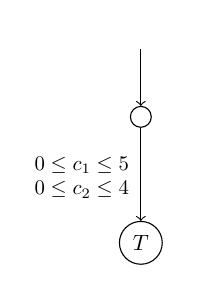
\begin{tikzpicture}[
		smallvertex/.style={circle,draw,scale=0.8}
		]
			
		\node[smallvertex](S0){ };
		\node[smallvertex, draw = none, above of = S0, yshift = 0.25cm](S4){};
		\draw[->] (S4) --(S0) node [midway, above, sloped, scale=0.75,
		rotate=295, xshift =-0.4 cm, yshift = -0.2cm]{};
		\node[smallvertex, below of = S0, yshift = -1cm](S3){$T$};
		\draw[->] (S0) edge (S3) node [midway, above, sloped, scale=0.75,		
		rotate=0, xshift =-1 cm, yshift = -1.5cm, align=center]{$0 \leq c_1 \leq 5$\\$ 0 \leq c_2 \leq 4$};
	\end{tikzpicture}
\end{subfigure}
%\end{center}
\caption{CMD representation}
\label{fig:cmd-example}
\end{figure}

\subsubsection{Zone BDD}
In ~\cite{7098276, 7184781} a method is proposed purely based on BDDs by translating the constraints directly into BDD nodes. We call this method BDD zones. This results in a unified structure for both the discrete variables and the clock constraints. The method is only a proof of concept and has not been implemented in a model checker and no performance results are known. Subsumption for this method may be difficult. On BDDs only equalities can be checked, and no inequalities. This way inclusion is not trivial to check by normal BDD algorithms.

\subsubsection{Digitization}
Digitization approximates the continuous values of clocks by using discrete values~\cite{CHARME01}. The method however, only works for closed timed automata, meaning that no strict comparisons on clocks can be made in the model and that clocks only can be compared to integers. This approach is very sensitive to the granularity of the values used and the upper bound of the clock values. When fine granularity or large upper bounds are used, the memory usage will increase too much. An advantage of this approach is that basic model checking approaches can be used and no extra complexity due to zone calculations is added. This method results in a transition system with only discrete variables, so a normal BDD package can be used. In ~\cite{nguyen2012discrete} a similar approach is proposed by using clock tick actions to represent time progress and removing clock variables altogether.

%\begin{table}[]
%\centering
%\caption{Comparing Diagrams}
%\label{table:diagrams}
%\begin{tabular}{|l|l|l|}
%\hline
%Type                                                   & Pro                                                                                                                                                                                                                             & Con                                                                                                                                                                                                                                                          \\ \hline
%DBM                                                    & \begin{tabular}[c]{@{}l@{}}Canonical form for convex zones\\ Existing library\\ Inclusion check\end{tabular}                                                                                                                    & \begin{tabular}[c]{@{}l@{}}Concave zones need multiple DBMs\\ Not memory efficient\end{tabular}                                                                                                                                                              \\ \hline
%DDD                                                    & \begin{tabular}[c]{@{}l@{}}Structure like LDD\\ Re-ordering of variables possible\\ Apply same efficiency as BDDs\\ Discrete variables also in DDD\end{tabular}                                                                  & \begin{tabular}[c]{@{}l@{}}Canonicity hard to obtain\\ No on the fly canonicity\\ Expensive normal form computation\\ Only time performance tested\\ Only reduction algorithms\end{tabular}                                                                  \\ \hline
%CDD                                                    & \begin{tabular}[c]{@{}l@{}}Structure like MDD\\ Inclusion check\\ (intersection of complement)\end{tabular}                                                                                                                     & \begin{tabular}[c]{@{}l@{}}No algorithm to get normal form\\ Only high level algorithms given\\ Methods don't maintain disjointness\\ Expensive normal form computation\\ No implementation results available\\ Disjointness memory inefficient\end{tabular} \\ \hline
%CRD                                                    & \begin{tabular}[c]{@{}l@{}}Combination with BDD possible\\ Variable reordering shows advantage\\ Library available\\ Some benchmarks exp better than CDD\\ Extensive benchmarks\\ Good performance backwards reach\end{tabular} & \begin{tabular}[c]{@{}l@{}}3 possible canonical forms\\ No algorithms in paper\\ Some benchmarks linear worse than CDD\end{tabular}                                                                                                                          \\ \hline
%CMD                                                    & Benchmarks against RED and \uppaal{} & \begin{tabular}[c]{@{}l@{}}Results differ per case\\ Needs translation from vector to edges\\ Two reduced forms\end{tabular}                                                                                                                                 \\ \hline
%\begin{tabular}[c]{@{}l@{}}BDD\\ discrete\end{tabular} & \begin{tabular}[c]{@{}l@{}}Using existing BDD packages\\ Good performance for small clock values\end{tabular}                                                                                                                   & \begin{tabular}[c]{@{}l@{}}Performance decreases fast for large values\\ Not possible with current Opaal \pins{}\\ Introducing additional 'tick' actions\\ Only for closed timed automata\end{tabular}                                                          \\ \hline
%\begin{tabular}[c]{@{}l@{}}BDD\\ zones\end{tabular}    & \begin{tabular}[c]{@{}l@{}}Using existing BDD packages\\ All variable reorderings possible\\ Only need direct translation DBM to\\ state vector\\ Easy to implement\end{tabular}                                                & \begin{tabular}[c]{@{}l@{}}Losing zone containment\\ No implementation results\end{tabular}                                                                                                                                                                  \\ \hline
%\end{tabular}
%\end{table}


\begin{table}
    \begin{tabular}{|l|llllllll|}
    \hline
                  & \rot{Reordering} & \rot{Subsumption} & \rot{Experiments} & \rot{Results} & \rot{Algorithms} & \rot{\begin{tabular}[c]{@{}l@{}}Canonical\\form\end{tabular}}& \rot{Similarity} & \rot{\begin{tabular}[c]{@{}l@{}}Connect with\\ other diagram\end{tabular}} \\ \hline
    DBM                  & -          & +           & +           & ~       & +          & +              & -          & ?                          \\
    DDD                  & +          & +           & time only   & +       & +/-        & hard           & LDD        & ?                          \\
    CDD                  & ?          & +           & -           & -       & +/-        & hard           & MDD        & ?                          \\
    CRD                  & +          & ?           & +           & +       & -          & 3 options      & MDD        & BDD                        \\
    CMD                  & -          & ?           & +           & +/-     & ~          & reduced        & -          & ?                          \\
    BDD discrete         & +          & -           & +           & +/-     & +          & +              & BDD        & BDD                        \\
    BDD zones            & +          & -           & -           & -       & +          & +              & BDD        & BDD                        \\ \hline
    \end{tabular}
\caption{Comparing Diagrams}
\label{table:diagrams}
\end{table}


\subsubsection{Orderings}
A known difficulty in BDDs is the variable ordering. A bad ordering can lead to a BDD of exponential size, where a good ordering can sometimes lead to a significantly smaller diagram. Of the zone diagrams named above, only for CRDs experiments with different orderings have been conducted, the other researches assume a given ordering on the variables and the ordering of the values is fixed. The CRD case shows that full interleaving and having related variables close to each other in the ordering is preferable, and gives the best results, both on speed and memory. This is the same result as expected with BDDs. This suggests that similar orderings should be used with these techniques. The techniques using normal BDDs can use standard BDD reorderings.

In Table \ref{table:diagrams} we compare the different types of diagrams we discussed above. We used different criteria. The table shows if reorderings are possible, if a subsumption check can be done, if experiments are done with the structure and their results, if canonical forms can be reached and how hard this is, if it is similar to a diagram for discrete variables, and if it can be connected to another type of diagram. The table uses $+$ and $-$ to express if a diagram has a certain property or not, $+/-$ is used for experiments and results if the experiments were limited or the results differ per test case. A $?$ is used when it is not clear if the diagram has a certain property or not. 

\begin{figure}[h] 
\input{pins}
\caption{Modular structure of \ltsmin{}~\cite{eemcs18152}}
\label{fig:pins_modern}
\end{figure}

\subsection{LTSmin}
\ltsmin{}~\cite{eemcs18152,ltsmin-mc:nmf2011} is a language independent model checker. It is built in a modular way such that new languages can be added by a \pins{} (Partitioned Next-State Interface) without too much effort, and new algorithms can be added easily. \ltsmin{} offers four different algorithmic back-ends for model analysis: symbolic, multi-core, sequential and distributed. All of these back-ends support different types of reduction and model checking. Several language modules have already been built for \ltsmin{} such as \mcrl{}, \promela{}, \dve{} and \uppaal{}. The modular structure of \ltsmin{} is shown in Figure \ref{fig:pins_modern}. The \pins{} is the core of \ltsmin{}. This interface abstracts as much as possible from the model without losing the structure. It represents states as fixed length integer arrays. The main function of the interface is a (partitioned) next-state function which returns the successor states. With these functions a state space can be generated on the fly. With the use of dependency matrices event locality can be determined statically~\cite{rwcmatrices}. With these matrices, more efficient symbolic algorithms can be used, the number of next-state calls can be reduced, efficient variable re-orderings can be used, and transition caching can be used. In the current \uppaal{} \pins{} the next-state function is not partitioned and therefore no meaningful dependency matrix is created, and none of these algorithms can be used. Also the DBM variable is only represented by a pointer, which is not a meaningful value for the transition system, as it is just a pointer, and does not contain information about the actual zone. \ltsmin{} uses the pointer to a DBM to do the subsumption check as described in section \ref{subsec:subsumtion}.

\subsubsection{Dependency Matrices}
To make use of most optimizations of symbolic model checking, a notion of event locality is used. In \ltsmin{} this is done by dependency matrices{rwcmatrices}. Dependencies can be divided into four types: read(r), must-write(w), may-write(W) and copy(-). When a variable is both may-write and read, a read/write dependency(+) is used. Each variable in the state-vector is represented, for each group, in this matrix. A read dependency is used when a variable is read in a group. The must-write dependency is used when a variable is always written, the may-write dependency is used when it may be written, but in some cases it can also be copied. This can occur, for example when a position in an array is written, or when the write happens inside a condition. The copy dependency is used when neither of the other dependencies applies. The variable will not change in this group. In Figure \ref{fig:dep_matrix} we show a dependency matrix of the two simple transition groups below.
\begin{center}
    \begin{tabular}{lll}
    1: & $x = 1 \vee a[2] = 0$ & $\rightarrow a[2] := 1, x:=0$  \\
    2: & $a[1] = 1$                     & $\rightarrow a[x] := 0, x:= 1$ \\
    \end{tabular}
\end{center}

\begin{figure}[h]
\centering
	\begin{math}
% 		\begin{pmatrix}
 \kbordermatrix{ 		               & x & a[0] & a[1] \cr
 									  1& + & -    & +    \cr
 									  2& w & +    & W    \cr}
% 		\end{pmatrix}
	\end{math}
	\caption{Dependency Matrix}
	\label{fig:dep_matrix}
\end{figure}

\subsection{Difference Decision Diagrams}

We have discussed several symbolic approaches for representing zones. All of these approaches have benefits and downsides over each other. We chose to develop one of these approaches in \ltsmin{}. We wanted a diagram that can store both discrete states and zones, this can either be done in the diagram, or in a combination of the diagram and BDD or LDD nodes. Also a subsumption check on the diagram should be possible. We chose from the four zone-representing diagrams discussed earlier. The CDD approach was not chosen due to the memory inefficient disjoint intervals and their algorithms not maintaining these disjointness. The CMD approach is too similar to DBMs, on which we already have an approach. The choice between CRD and DDD was between two quite similar diagrams. We have decided to continue on the DDD. It is a diagram form that is closely related to LDDs, for which we already have a library, so we can reuse parts of the LDD library, and it is also quite compatible with the current \pins{} structure and its next-state function, so no big changes are needed for that. A translation from a path in a DDD structure into a state-vector used by \ltsmin{} can be made without too much effort. %The method still has some loose ends that need research, mostly on the algorithms and efficiently creating a canonical form. No results on the memory usage are available, which is normally the greatest benefit of a symbolic approach, so also on the results side we can extend the current research. 

So DDDs are a diagram type that seems to fit well in the current structure we have. We already defined a DDD in the previous subsection. We will now also give the semantics of this structure. The semantics uses the if-then-else operator, denoted by $\rightarrow$.

\begin{mydef}[DDD semantics]
\label{def:Semantics1}
The semantics of a vertex is defined recursively by the function $\mathcal{V}: V \rightarrow \textbf{Exp}:$
\begin{itemize}
\item $\mathcal{V}[[0]] \myeq$ false,
\item $\mathcal{V}[[1]] \myeq$ true,
\item \begin{math} \mathcal{V}[[v]] \myeq
\begin{cases}
(pos(v) - neg(v) < const(v)) \rightarrow \mathcal{V}[[high(v)]],\mathcal{V}[[low(v)]]\text{if }op(v) = '<'\\
(pos(v) - neg(v) \leq const(v)) \rightarrow \mathcal{V}[[high(v)]],\mathcal{V}[[low(v)]]\text{if }op(v) = '\leq'
\end{cases}
\end{math}
\end{itemize}
\end{mydef}

In the semantics we only take the information on the high edges. The implicit information on the low edge is not used. A node can only represent an upper-bound which is either true or false, it cannot implicitly represent a lower-bound on the same variable pair. This representation also makes it easier to work with the state-vectors of \ltsmin{}.

In~\cite{ddds} a canonical form for DDDs is discussed, also called a fully reduced DDD. Only definitions are given here, no algorithms to reach this form. It is stated that it is difficult to reach this fully reduced form. It is not clear if they managed to make their apply function in such a way that it maintains canonicity, as the function for BDDs does. To reach canonicity, local reductions and ordering are a first step, but it is not enough due to dependencies among the constraints. For BDDs the local reductions and ordering are sufficient to reach a canonical form. First, we give some notational shorthands and then we define an ordering and local reductions on DDDs.
%
\begin{center}
\begin{tabular}{lll}
$var(v)$   & $=$ & $(pos(v),neg(v))$   \\
$bound(v)$ & $=$ & $(const(v),op(v))$  \\
$cstr(v)$  & $=$ & $(var(v),bound(v))$
\end{tabular}
\end{center}

To order DDD nodes we use the operator $\prec$. This orders variables and variable pairs in a predefined order. It orders bounds by increasing constants, and the $<$ operator before the $\leq$ operator. So a node $v$ with $bound(v) = (0,<)$ comes before $bound(u) = (0,\leq)$ which comes before $bound(w) = (1,<)$.

\begin{mydef}[Ordered DDD~\cite{ddds}]
\label{def:ODDD}
An ordered DDD (ODDD) is a DDD where each non-terminal vertex $v$ satisfies:
\begin{enumerate}
  \item $neg(v) \prec pos(v)$,
  \item $var(v) \prec var(high(v))$,
  \item $var(v) \prec var(low(v))$ or \\ $var(v) = var(low(v))$ and $bound(v) \prec bound(low(v))$.
\end{enumerate}
\end{mydef}

After ordering a DDD some local reductions can be defined to reduce the size of a DDD.

\begin{mydef}[Locally Reduced DDD~\cite{ddds}]
\label{def:RLDDD}
A locally reduced DDD ($R_LDDD$) is an ODDD satisfying, for all non-terminals u and v:
\begin{enumerate}
  \item $\mathbb{D} = \mathbb{Z}$ implies $\forall v. op(v) = '\leq'$,
  \item $(cstr(u),high(u),low(u)) = (cstr(v),high(v),low(v))$ implies $u = v$,
  \item $low(v) \neq high(v)$,
  \item $var(v) = var(low(v))$ implies $high(v) \neq high(low(v))$.
\end{enumerate}
\end{mydef}

We give an example of the last point in figure \ref{fig:rlddd}. Here both diagrams represent the same zone: $2 < c_1 - c_2 \leq 8$. The node with $< 4$ on the high edge is redundant in this example and can thus be removed. We do not strictly test for the first rule. Even if we only use integer comparisons, we will also represent strict comparisons. The values of clocks are real, and not integer, so there is a difference between both operators.

\begin{figure}[h]
\begin{center}
	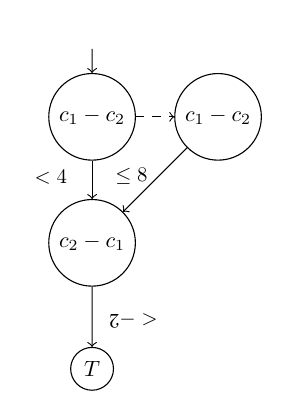
\begin{tikzpicture}[
		smallvertex/.style={circle,draw,scale=0.8}
		]
			
		\node[smallvertex](S0){$c_1 - c_2$};
		\node[smallvertex, draw = none, above of = S0, yshift = 0.25cm](S5){};
		\draw[->] (S5) --(S0) node [midway, above, sloped, scale=0.75,
		rotate=295, xshift =-0.4 cm, yshift = -0.2cm]{};
		\node[smallvertex, right of = S0, xshift = 1cm](S1){$c_1 - c_2$};
		\draw[dashed,->] (S0) --(S1) node [midway, above, sloped, scale=0.75,
		rotate=0, xshift =-0.7 cm, yshift = -0.2cm]{};
		\node[smallvertex, below of = S0, yshift = -1cm](S2){$c_2 - c_1$};
		\draw[->] (S0) --(S2) node [midway, above, sloped, scale=0.75,
		rotate=90, xshift =-0.7 cm, yshift = -0.2cm]{$< 4$};
		\draw[->] (S1) --(S2) node [midway, above, sloped, scale=0.75,
		rotate=315, xshift =-0.4 cm, yshift = -0.2cm]{$\leq 8$};
		\node[smallvertex, below of = S0, yshift = -3cm](S4){$T$};
		\draw[->] (S2) --(S4) node [midway, above, sloped, scale=0.75,
		rotate=90, xshift =-0.7 cm, yshift = -0.2cm]{$<-2$};
	\end{tikzpicture}
	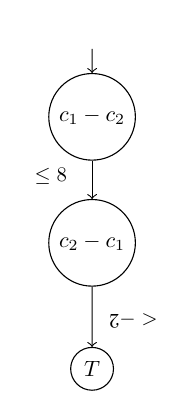
\begin{tikzpicture}[
		smallvertex/.style={circle,draw,scale=0.8}
		]
			
		\node[smallvertex](S0){$c_1 - c_2$};
		\node[smallvertex, draw = none, above of = S0, yshift = 0.25cm](S5){};
		\draw[->] (S5) --(S0) node [midway, above, sloped, scale=0.75,
		rotate=295, xshift =-0.4 cm, yshift = -0.2cm]{};
		\node[smallvertex, below of = S0, yshift = -1cm](S2){$c_2 - c_1$};
		\draw[->] (S0) --(S2) node [midway, above, sloped, scale=0.75,
		rotate=90, xshift =-0.7 cm, yshift = -0.2cm]{$\leq 8$};
		\node[smallvertex, below of = S0, yshift = -3cm](S4){$T$};
		\draw[->] (S2) --(S4) node [midway, above, sloped, scale=0.75,
		rotate=90, xshift =-0.7 cm, yshift = -0.2cm]{$<-2$};
	\end{tikzpicture}
\end{center}
\caption{Local reduction}
\label{fig:rlddd}
\end{figure}

For BDDs these reductions would be enough to have a fully canonical structure. For DDDs this is not the case, due to dependencies between the bounds. In Figure \ref{fig:non-canonical} we give an example for this by giving two different locally reduced DDDs representing the same zone. The resulting zone of both these DDDs is drawn in Figure \ref{fig:non-canonical-zone}, which is the square in which both clock $c_1$ and $c_2$ are between 0 and 5.

\begin{figure}[h]
\begin{center}
	\begin{subfigure}{0.3\textwidth}
	\begin{tikzpicture}[
		smallvertex/.style={circle,draw,scale=0.8}
		]
		\node[smallvertex, draw = none, above of = S0, yshift = 0.25cm](S0){};
		\node[smallvertex](S1){$\mathbf{O} - c_1$};
		\node[smallvertex, below of = S1, yshift = -1cm](S2){$\mathbf{O} - c_2$};
		\node[smallvertex, below of = S2, yshift = -1cm](S3){$c_1 - \mathbf{O}$};
		\node[smallvertex, below of = S3, yshift = -1cm](S4){$c_1 - c_2$};
		\node[smallvertex, below of = S4, yshift = -1cm](S5){$c_2 - \mathbf{O}$};
		\node[smallvertex, below of = S5, yshift = -1cm](S6){$c_2 - c_1$};
		\node[smallvertex, below of = S6, yshift = -1cm](S7){$T$};
		
		\draw[->] (S0) --(S1) node [midway, above, sloped, scale=0.75,
		rotate=0, xshift =-0.4 cm, yshift = -0.2cm]{};
		\draw[->] (S1) --(S2) node [midway, above, sloped, scale=0.75,
		rotate=90, xshift =-0.4 cm, yshift = -0.2cm]{$<0$};
		\draw[->] (S2) --(S3) node [midway, above, sloped, scale=0.75,
		rotate=90, xshift =-0.4 cm, yshift = -0.2cm]{$<0$};
		\draw[->] (S3) --(S4) node [midway, above, sloped, scale=0.75,
		rotate=90, xshift =-0.4 cm, yshift = -0.2cm]{$<5$};
		\draw[->] (S4) --(S5) node [midway, above, sloped, scale=0.75,
		rotate=90, xshift =-0.4 cm, yshift = -0.2cm]{$<\infty$};
		\draw[->] (S5) --(S6) node [midway, above, sloped, scale=0.75,
		rotate=90, xshift =-0.4 cm, yshift = -0.2cm]{$<5$};
		\draw[->] (S6) --(S7) node [midway, above, sloped, scale=0.75,
		rotate=90, xshift =-0.4 cm, yshift = -0.2cm]{$<\infty$};
		
	\end{tikzpicture}
	\end{subfigure}
	\begin{subfigure}{0.3\textwidth}
	\begin{tikzpicture}[
		smallvertex/.style={circle,draw,scale=0.8}
		]
		\node[smallvertex, draw = none, above of = S1, yshift = 0.25cm](S0){};
		\node[smallvertex](S1){$\mathbf{O} - c_1$};
		\node[smallvertex, below of = S1, yshift = -1cm](S2){$\mathbf{O} - c_2$};
		\node[smallvertex, below of = S2, yshift = -1cm](S3){$c_1 - \mathbf{O}$};
		\node[smallvertex, below of = S3, yshift = -1cm](S4){$c_1 - c_2$};
		\node[smallvertex, below of = S4, yshift = -1cm](S5){$c_2 - \mathbf{O}$};
		\node[smallvertex, below of = S5, yshift = -1cm](S6){$c_2 - c_1$};
		\node[smallvertex, below of = S6, yshift = -1cm](S7){$T$};
		
		\draw[->] (S0) --(S1) node [midway, above, sloped, scale=0.75,
		rotate=0, xshift =-0.4 cm, yshift = -0.2cm]{};
		\draw[->] (S1) --(S2) node [midway, above, sloped, scale=0.75,
		rotate=90, xshift =-0.4 cm, yshift = -0.2cm]{$<0$};
		\draw[->] (S2) --(S3) node [midway, above, sloped, scale=0.75,
		rotate=90, xshift =-0.4 cm, yshift = -0.2cm]{$<0$};
		\draw[->] (S3) --(S4) node [midway, above, sloped, scale=0.75,
		rotate=90, xshift =-0.4 cm, yshift = -0.2cm]{$<5$};
		\draw[->] (S4) --(S5) node [midway, above, sloped, scale=0.75,
		rotate=90, xshift =-0.4 cm, yshift = -0.2cm]{$<5$};
		\draw[->] (S5) --(S6) node [midway, above, sloped, scale=0.75,
		rotate=90, xshift =-0.4 cm, yshift = -0.2cm]{$<5$};
		\draw[->] (S6) --(S7) node [midway, above, sloped, scale=0.75,
		rotate=90, xshift =-0.4 cm, yshift = -0.2cm]{$<5$};
		
	\end{tikzpicture}
	\end{subfigure}
\end{center}
\caption{Two DDDs representing the same zone}
\label{fig:non-canonical}
\end{figure}

\begin{figure}[h]
\centering
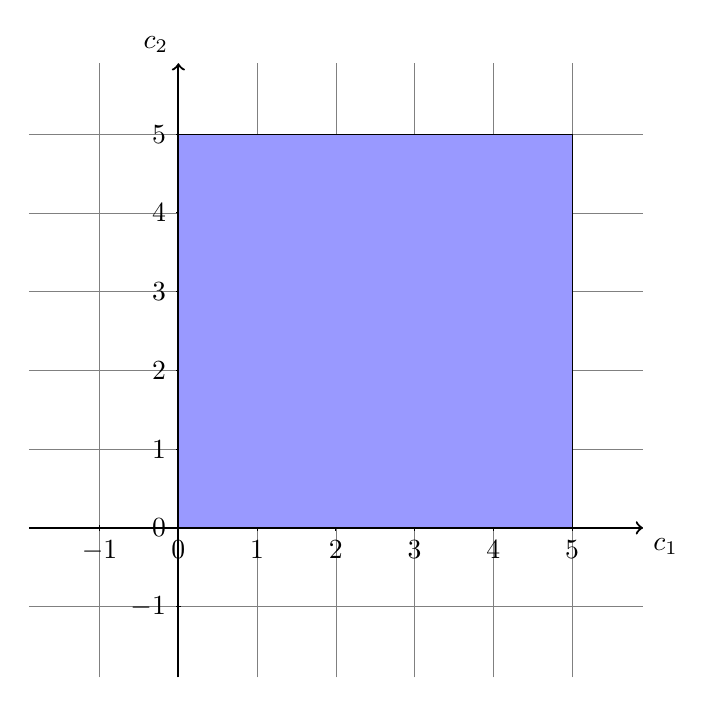
\begin{tikzpicture}

\draw[step=1cm,gray,very thin] (-1.9,-1.9) grid (5.9,5.9);

%\shadedraw[inner color=blue,outer color=red, draw=black] (0,0) rectangle (4,4);

\draw[thick,->] (-1.9,0) -- (5.9,0) node[anchor=north west] {$c_1$};
\draw[thick,->] (0,-1.9) -- (0,5.9) node[anchor=south east] {$c_2$};

\foreach \x in {-1,0,1,2,3,4,5}
    \draw (\x cm,1pt) -- (\x cm,-1pt) node[anchor=north] {$\x$};
\foreach \y in {-1,0,1,2,3,4,5}
    \draw (1pt,\y cm) -- (-1pt,\y cm) node[anchor=east] {$\y$};
    
\filldraw[fill=blue!40!white, draw=black] (0,0) rectangle (5,5);
\end{tikzpicture}
\caption{Resulting zone of DDDs in figure \ref{fig:non-canonical}}
\label{fig:non-canonical-zone}
\end{figure}

The $R_LDDD$ is clearly not canonical. First, we define a path in a DDD as the bound on all high edges that are traversed in a single walk from the top node to the true node. A path $[p]$ will only have one bound for each variable pair.

\begin{mydef}[Path-reduced DDD~\cite{ddds}]
A path-reduced DDD ($R_PDDD$) is a locally reduced DDD where all paths are feasible.
\end{mydef}

This definition ensures that all paths in a DDD actually represent a zone, and that there are no redundant paths in the DDD that just represent an empty set. This usage of paths is compatible to the state vectors used in \ltsmin{}. An $R_PDDD$ is still not canonical. We need to define tightness, saturation and disjunctive vertices. To define tightness we first need to define dominating constraints.

\begin{mydef}[Dominating constraint~\cite{ddds}]
A constraint $x_i - x_j \lesssim c$ is dominating in a path $[p]$ if all other constraints $x_i - x_j \lesssim' c'$ on the same pair of variables in $p$ are less restrictive.
\end{mydef}

\begin{mydef}[Tightness~\cite{ddds}]
A dominating constraint $\alpha = x_i - x_j \lesssim c$ is tight in a feasible path $[p] = [p_1] \wedge \alpha \wedge [p_2]$ if for all tighter constraints $(c', \lesssim') < (c,\lesssim),$ the systems $[p_1] \wedge (x_i - x_j \lesssim' c') \wedge [p_2]$ and $[p]$ have different solutions. A path $p$ is tight if it is feasible and all dominating constraints on it are tight. An $R_LDDD u$ is tight if all paths from $u$ are tight. 
\end{mydef}

\begin{mydef}[Saturation~\cite{ddds}]
A tight path $p$ from an $R_PDDD$ is saturated if for all constraints $\alpha$ not on $p$, if $\alpha$ is added to $p$ either (1) $\alpha$ is not dominating and tight, or (2) the constraint system $[p_1] \wedge \neg\alpha$ is infeasible when $[p]$ is written $[p] = [p_1] \wedge [p_2]$ with all constraints on $p_1$ smaller than $\alpha$ with respect to $\prec$ and all constraints on $p_2$ larger than $\alpha$. An $R_PDDD$ $u$ is saturated if all paths from $u$ are saturated.
\end{mydef}

\begin{mydef}[Disjunctive vertex~\cite{ddds}]
Let $p$ be a path leading to the vertex $u$ in a DDD, and assume $\alpha = cstr(u), h = high(u),$ and $l = low(u)$. Then $u$ is disjunctive in $p$ if $[p] \wedge (\alpha \rightarrow h,l)$ and $[p] \wedge (h \vee l)$ have the same set of solutions.
\end{mydef}

All of these definitions together lead to the following definition of a fully reduced DDD.
 
\begin{mydef}[Fully reduced DDD~\cite{ddds}]
\label{def:RFDDD}
An $R_pDDD$ u is a fully-reduced DDD ($R_FDDD$) if it is tight, saturated and has no disjunctive vertices.
\end{mydef}

We assume that this fully-reduced DDD is canonical and work from that. It is not ensured that this is actually the case, there is no proof for it.

\begin{myconjecture}[Canonical DDD~\cite{ddds}]
\label{def:Canonical-ddd}
If $u$ and $v$ are $R_FDDDs$ with the same set of solutions then $u = v$.
\end{myconjecture}


DDDs can also be used to represent the discrete variables in automata. This is done by translating the variable into a difference constraint. For example $x_1 = 3$ will be translated into $x_1 - 0 \leq 3 \wedge 0 - x_1 \leq -3$, thus resulting into a DDD with two nodes. We will instead connect the DDD to an LDD to represent discrete variables to limit the number of nodes.

So far we only found the results of two benchmark tests of DDDs, Milner's scheduler and Fischer's protocol~\cite{Møller200253}. Here the DDD approach has been compared with KRONOS and \uppaal{} which were both slower than the DDD implementation. The results of these benchmarks show no memory usage or number of nodes needed.

\subsection{List Decision Diagram}
We will introduce the LDD structure here~\cite{sylvan}. An LDD is used to represent variables with integer values, not only binary values. In contrast to MDDs\cite{129849}, which have multiple outgoing edges per node, this is done for one value per node, resulting in nodes with equal size. We will first define the LDD structure.

\begin{figure}
\centering
	\begin{tikzpicture}[
		smallvertex/.style={circle,draw,scale=0.8}
		]
		\node[smallvertex, draw = none, above of = S1, yshift = 0.25cm](S0){};
		\node[smallvertex](S1){$a$};
		\node[smallvertex, below of = S1, yshift = -.5cm](S2){$b$};
		\node[smallvertex, below of = S2, yshift = -.5cm](S3){$c$};
		\node[smallvertex, below of = S3, yshift = -.5cm](S4){$d$};
		\node[smallvertex, below of = S4, yshift = -.5cm](S5){$T$};
		\node[smallvertex, right of = S2](S6){$b$};
		\node[smallvertex, right of = S3](S7){$c$};
		\node[smallvertex, right of = S6](S9){$b$};
		\node[smallvertex, above of = S9, yshift = .5cm](S8){$a$};
		\node[smallvertex, below of = S9, yshift = -.5cm](S10){$c$};
		\node[smallvertex, below of = S10, yshift = -.5cm](S11){$d$};
		
		\draw[->] (S0) --(S1) node [midway, above, sloped, scale=0.75,
		rotate=0, xshift =-0.4 cm, yshift = -0.2cm]{};
		\draw[->] (S1) --(S2) node [midway, above, sloped, scale=0.75,
		rotate=90, xshift =-0.4 cm, yshift = -0.2cm]{$0$};
		\draw[->] (S2) --(S3) node [midway, above, sloped, scale=0.75,
		rotate=90, xshift =-0.4 cm, yshift = -0.2cm]{$0$};
		\draw[->] (S3) --(S4) node [midway, above, sloped, scale=0.75,
		rotate=90, xshift =-0.4 cm, yshift = -0.2cm]{$0$};
		\draw[->] (S4) --(S5) node [midway, above, sloped, scale=0.75,
		rotate=90, xshift =-0.4 cm, yshift = -0.2cm]{$0$};
		\draw[dashed, ->] (S2) --(S6) node [midway, above, sloped, scale=0.75,
		rotate=90, xshift =-0.4 cm, yshift = -0.2cm]{};
		\draw[->] (S6) --(S7) node [midway, above, sloped, scale=0.75,
		rotate=90, xshift =-0.4 cm, yshift = -0.2cm]{$2$};
		\draw[->] (S7) --(S4) node [midway, above, sloped, scale=0.75,
		rotate=300, xshift =0.4 cm, yshift = -0.2cm]{$3$};
		\draw[dashed, ->] (S1) --(S8) node [midway, above, sloped, scale=0.75,
		rotate=90, xshift =-0.4 cm, yshift = -0.2cm]{};
		\draw[->] (S8) --(S9) node [midway, above, sloped, scale=0.75,
		rotate=90, xshift =-0.4 cm, yshift = -0.2cm]{$2$};
		\draw[->] (S9) --(S10) node [midway, above, sloped, scale=0.75,
		rotate=90, xshift =-0.4 cm, yshift = -0.2cm]{$0$};
        \draw[->] (S10) --(S11) node [midway, above, sloped, scale=0.75,
		rotate=90, xshift =-0.4 cm, yshift = -0.2cm]{$3$};
		\draw[->] (S11) --(S5) node [midway, above, sloped, scale=0.75,
		rotate=320, xshift =-0.4 cm, yshift = -0.2cm]{$1$};


	\end{tikzpicture}
\caption{LDD representation}
\label{fig:ldd-example}
\end{figure}

\begin{mydef}[List Decision Diagram]
\label{def:LDD}
A List Decision Diagram (LDD) is a directed acyclic graph $(V,E)$. The vertex set $V$ contains two terminals $0$ and $1$ with out-degree zero, and a set of non-terminal vertices with out-degree two and the following attributes.
\\\\
\begin{tabular}{lll}
Attribute                & Type                      & Description                                           \\\hline
var(v)                   & \textbf{Var}              & Variable x \\

const(v)                 & $\mathbb{Z}$              & Constant c.                                           \\
high(v), low(v)          & $V$                       & High-branch h, and low-branch l.                   
\end{tabular}
\captionof*{table}{}  
The set E contains the edges $(v,low(v))$ and $(v, high(v))$, where $v \in V$ is a non-terminal vertex.
\end{mydef} 

The definition is almost equal to DDDs, Definition \ref{def:DDD}. The difference is the operator that is not in LDDs. LDDs can be seen as a DDD with not a $<$ or $\leq$ as operator, but a $=$. The semantics of this diagram are again similar to those of DDDs, which can be defined using the if-then-else operator. 



\begin{mydef}[LDD semantics]
\label{def:LDDSemantics}
The semantics of a vertex is defined recursively by the function $\mathcal{V}: V \rightarrow \textbf{Exp}:$
\begin{itemize}
\item $\mathcal{V}[[0]] \myeq$ false,
\item $\mathcal{V}[[1]] \myeq$ true,
\item \begin{math} \mathcal{V}[[v]] \myeq
(var(v) = const(v)) \rightarrow \mathcal{V}[[high(v)]],\mathcal{V}[[low(v)]]\\
\end{math}
\end{itemize}
\end{mydef}

We give an example of an LDD in Figure \ref{fig:ldd-example} which represents the following values: $\{0,0,0,0\}, \{0,2,3,0\}, \{2,0,3,1\}$, for the vector $\{a,b,c,d\}$.

